\chapter{绪\hskip 0.4cm 论}
\label{ch1}

\section{研究背景及意义}
随着机器学习的不断发展和壮大,我们一方面惊叹于它的成就,比如Alpha GO击败了围棋世界冠军——柯洁、面部识别技术帮助我们抓住了躲藏多年的逃犯、大型工业企业也大力应用机器学习技术推动生产力的快速发展;另一方面,我们也认识到,机器学习还有巨大的发展潜力,例如:在医疗建设方面,构建基于大量病例的医疗救助诊断系统;在金融建设方面,运行基于大量商业行为数据的信用风险控制模型,帮助高价值的企业融资,并基于整个产业链的数据提供个性化的产品分配和营销策略。我们在各行各业真正见证了人工智能(AI)的巨大潜力,以及已经开始期待在许多应用中使用更复杂、更尖端的人工智能技术,包括无人驾驶、医疗、金融等。今天,人工智能技术几乎在各方面都大显身手。传统的人工智能系统依赖于集中管理的训练数据集,建立在大量数据上,从数据中学习特征,从而完成复杂的任务,甚至是人类也难以完成的操作。

人工智能的基础是大数据,而大多数训练数据是来自于不同组织的个人或机构。在一个深度学习的项目中,可能涉及到多个领域,需要采集不同公司、不同机构、不同部门的数据进行融合。(比如研究用户的消费爱好和水平,可能需要采集各个消费平台、银行、商店等多个机构的数据),然而在现实生活中,数据是分散在各地的,很难进行整合。于是诞生了集中式深度学习,它是通过收集数据并将其发送到一个能看到并控制所有数据的中央服务器,完成所有训练数据的整合。这个中心位置不仅要有强大的计算机集群来训练和创建深度学习模型,还要处理敏感数据并防止数据被用于其他目的。此外,敏感数据的处理方式必须不损害用户的隐私。集中式的深度学习需要大量的数据去训练模型,达到较好的训练效果。比如,大量的互联网公司从数百万的用户那里收集数据,然后利用这些数据进行深度学习,实现智能推荐、语音识别、面部识别等。然而在集中式深度学习中,中央服务器是半可信的,半可信是指服务器是诚实但好奇的(Honest but Curious),在处理一些敏感数据时,用户也不知道他们的数据将被用于何处,用户隐私安全存在一定的威胁。

而且,这些数据的采集很可能涉及到用户的隐私。在2018年,中国互联网协会收到用户举报发现,腾讯音乐等多家应用软件以“通过深度学习向用户提供更好的服务”为由,长期收集并保存大量的用户个人数据,如照片、地址、电话等,甚至将这些包含了用户大量个人隐私的数据用作其他途径,为企业谋取更多利益。资料显示,许多应用软件在数据收集方面存在大量的安全漏洞,比如,过度用户手机中的“通讯录”、“位置”、“麦克风”等信息,未经授权访问用户的本地数据,导致千万级的用户资料泄露。

随着越来越多的涉及数据泄漏和隐私侵权事件的发酵,人们的隐私意识的普遍提高,越来越的用户关注自己的隐私信息是否在未经个人许可,或者出于商业和政治目的被他人或机构利用。更多的用户拒绝向互联网企业提供“收集数据”的权限,关闭了“通讯录”、”短信“、“位置”等访问权限。同时,相关的隐私法律法规不断完善,中国出台的《网络安全与数据合规》白皮书中明确要求加强用户个人信息保护,2018年欧洲联盟会出台的《通用数据保护条例》强调保护用户的隐私和数据的使用安全性。随着个人意识和国家政策的关注,在大数据和人工智能领域数据采集和使用的过程中,保护用户隐私和数据的机密显得越来越重要。

人工智能的力量是基于大数据的,在数据监管和隐私保护的要求下,传统的集中式深度学习系统难以收集到模型训练所需要的数据,进而无法提供更专业的网络服务。大数据的基础没有了,人工智能的未来也就岌岌可危。那么能否创建一个深度学习框架,使人工智能系统能够更有效和准确地集体使用数据,同时满足隐私性、安全性和监管要求,并解决数据孤岛的问题。如何才能做到这一点呢?

为了解决这个问题,google在2016年率先提出了联邦学习的概念\upcite{ref3},它提供了一个具有隐私保护功能的分布式深度学习框架,该框架通过分布式的方式使成千上万的参与者协作,共同迭代训练一个联合的深度学习模型。这种机制允许参与者之间共享训练模型,但是训练数据在联合训练过程中仅保存在参与者的本地,确保了每个参与者的隐私。

如图\ref{fig:联邦学习模型概况}所示,联邦学习的基本工作流程如下:
\begin{itemize}
\item \textbf{初始化:}所有用户在他们的设备上都有一个预先分配的神经网络模型,并且可以自愿加入联邦学习协议,指定相同的深度学习和模型训练目标。
\item  \textbf{本地训练:}在一个给定的通信回合中,联邦学习参与者首先从中央服务器下载全局模型参数,然后使用他们的私人训练模式训练模型,更新本地模型(即模型参数),并将这些更新发送到中央服务器。
\item \textbf{中央参数聚合:}中央服务器汇总此次通信回合中所有参与者上传的模型参数,并对其进行聚合求得全局模型的参数,然后更新全局模型。
\item \textbf{迭代更新:}迭代地执行上述步骤直至全局模型参数满足收敛条件,最终得到最优的全局模型。
\end{itemize}

\begin{figure}[!hbt]
\centering
	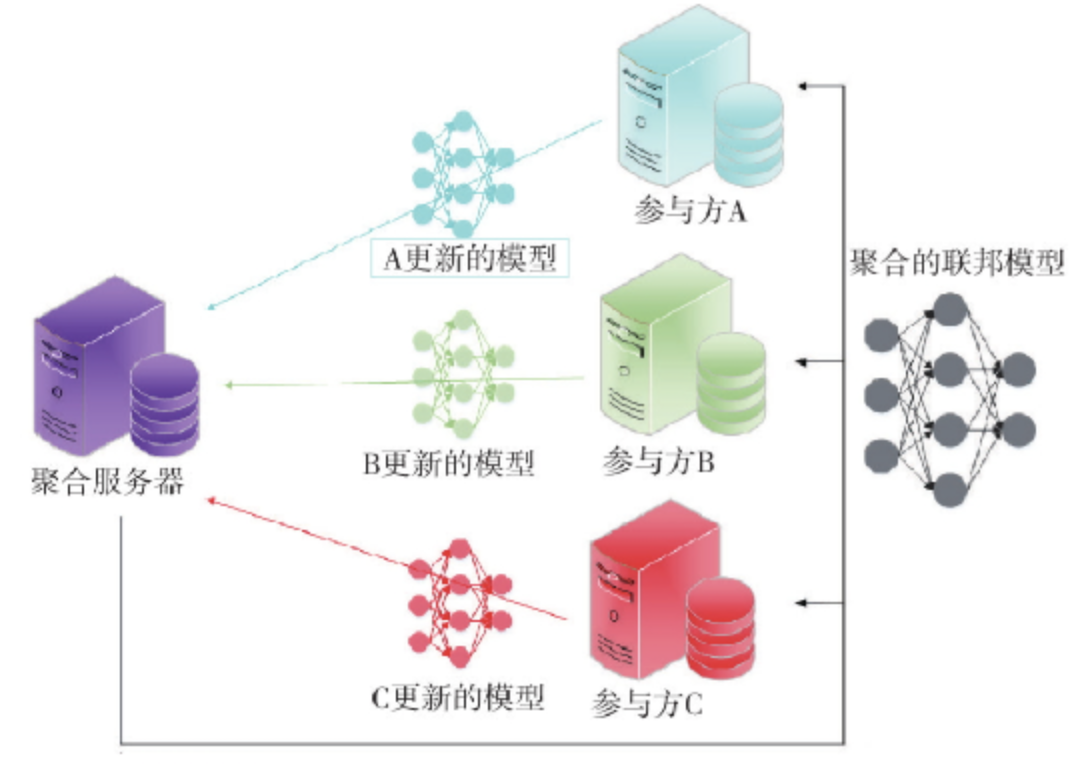
\includegraphics[scale=0.5]{fig2/C1/联邦学习概况}%联邦学习的系统架构
	\caption{联邦学习模型概况}
	\label{fig:联邦学习模型概况}	
\end{figure}

联邦学习在隐私敏感的场景(包括金融、工业和许多其他与数据相关的场景)中展现出巨大的前景,这是因为它具有独特的优势,多个参与者无需共享本地数据却能训练出统一的全局模型,保护了本地数据的隐私性\upcite{ref4}。联邦学习解决了数据聚合的问题,并允许一些机器学习模型和算法在各机构和部门之间进行独立设计和训练。在一些移动设备上的机器学习模型应用中,联邦学习展示出良好的性能和稳健性。此外,对于一些没有足够的私人数据来训练准确的本地模型的用户(客户)来说,深度学习模型和算法的性能可以通过联邦学习得到显著改善。

\section {问题和挑战}
\subsection{数据异构}
由于联邦学习的重点是通过以分布式方式从所有参与的客户端设备中学习本地数据来获得高质量的全局模型,所以它无法捕捉每个设备的个人信息,导致推理或分类性能下降。此外,传统的联邦学习要求所有参与的设备同意使用一个共同的模型来共同训练,这在复杂的现实世界物联网应用中是不现实的。研究人员对联邦学习在实际应用中面临的问题总结如下\upcite{ref5}:

(1)设备的异质性:由于客户端设备的硬件条件(CPU、内存)、网络连接(3G、4G、5G、WiFi)和电源(电池)的变化,联邦学习网络上每个设备的通信、存储和计算能力都可能有差异。受限于网络和设备,不能保证在任何时候所有设备都能参与学习。此外,设备可能会受到意外事件的影响,如断电或断网,这可能会导致暂时的断网。这种异质性的系统结构影响了联邦模型的整体学习战略。

(2)统计的异质性:在整个网络中,设备通常以不同的方式产生和收集数据,而且不同设备的数据量、特征等会有很大的不同,所以联邦学习网络中的数据不是独立和相同的分布(非IID)。目前的深度学习算法主要是基于IID数据。因此,非IID数据的异质属性给建模、分析和评估带来了重大挑战。联邦学习的参数聚合FedAvg)方法可以解决非均匀同分布数据的问题,但是当数据分布偏态很严重的时候FedAvg的性能退化严重,一方面其性能比中心化的方法差好多,另一方面它只能学习到IoT设备粗粒度的特征而无法学习到细粒度的特征。

(3)模型的异质性:每个客户根据其应用场景要求定制不同模型。

\subsection{高昂的通信代价}
在联邦学习过程中,根据存储在几十甚至几百万个远程客户端设备上的数据来学习一个全局模型。原始数据被储存在本地的客户端设备上,在训练过程中这些远程设备必须不断地与中央服务器互动,以完成全局模型的构建。通常情况下,整个联盟学习网络可能涉及大量的设备,而网络通信可能比本地计算慢几个数量级,因此高通信成本成为联邦学习的关键瓶颈。

\subsection{安全性和隐私威胁}
联邦学习解决了传统集中式深度学习所面临的大规模数据收集等问题,减少了数据在收集过程中所遇到的隐私泄露风险,节省了传输数据所占用的通信资源。但是,联邦学习中的共享参数以及传输数据的无线链路仍然可能泄露数据隐私。

在联邦学习系统中,攻击方可能是内部攻击者,比如中央服务器、本地客户端;也有可能是外部攻击者。他们试图影响、破坏联邦学习模型的准确性,恶意推导本地客户端的训练数据。外部攻击主要通过本地客户端与中央服务器之间的通信信道发起。

有一些恶意参与者会发送无效的模型参数更新到中央服务器,破坏全局模型的训练。比如,这些恶意参与方作为本地客户端参加训练,修改本地的训练数据,对本地数据注入一些有毒的数据,进行投毒攻击,从而损害全局模型的准确性,操纵模型的预测结果。

在训练过程中,局部模型更新和全局模型参数的结合过程,提供了关于训练数据的隐藏知识,用户的个人信息很有可能泄露给不受信任的服务器或其他恶意用户。例如,白盒推理攻击和黑盒推理攻击通过客户端上传的参数恶意的窃取用户的训练数据生成的样本原型。

\section{国内外研究现状}
尽管联邦学习框架提供了隐私保护的机制,还是有各种类型的攻击方式可以攻击联邦学习系统,从而破坏联邦学习系统安全和参与方的隐私。本节将重点讨论关于联邦学习的攻击模型和隐私保护的研究现状。

\subsection{攻击模型的研究现状}
各类攻击模型阻碍了深度学习技术的发展,也会极大地威胁到人们的隐私敏感信息。无论是模型并行化还是数据并行化,分布式学习系统在用户数据隐私性方面相对于集中式学习存在一定的优势 。但文献\upcite{ref6}的作者发现, 在分布式联邦学习系统中, 参与者需要多次的联合迭代过程才能完成全局模型的收敛, 参与者的参数也需要多次的训练、上传和共享, 这些参数中包含的参与者训练集的相关信息, 用户的信息可以通过计算用户上传的多个参数得到。因此,有许多外部攻击者或者恶意服务器通过用户上传的参数恢复出原始的样本试例。

模型反演攻击:\upcite{ref7}利用用户上传的参数信息,以一种很简单的方式攻击用户数据:一旦用户的网络模型经过训练并达到收敛,攻击者就可以通过调整网络模型权重的梯度, 获得网络模型中所有表示类的逆向工程试例。在模型反演攻击中, 攻击者无需接触目标信息的标签类,攻击模型仍然能够恢复原始样本试例。这一攻击模型表明,任何经过精确训练的深度学习网络,无论是以何种方式进行训练收敛, 都可以泄露深度网络中区分不同标签类的信息。但是参数中包含的信息有限,模型反演攻击方式很难攻击卷积神经网络等复杂深度网络模型,在模型进行了一定的隐私保护后,攻击也基本失效。

生成对抗攻击(GAN攻击):目前研究人员也利用诸多安全模型对深度学习网络的训练数据集进行保护,但Hitaj等人\upcite{ref8}发现,一个联邦学习框架非常容易受到系统内参与者发起的主动攻击。他们首次提出了基于GAN的模型重建攻击,攻击者为本地客户端。在训练阶段,攻击者冒充为本地的无害用户,训练GAN模型,模拟产生其他用户的训练数据产生的原型样本,之后通过不断添加假的训练样本,攻击可以逐渐影响整个学习过程,使受害者暴露出更多关于被攻击者的目标类的敏感信息。除了客户端发起的GAN攻击,服务器也能通过GAN攻击。恶意服务器最初假装是一个为用户提供联邦学习服务的正常服务器,其主要目标是重建被攻击用户的训练样本。

投毒攻击:在联邦学习框架中,攻击者可能试图修改、删除或插入恶意信息到训练数据中,以破坏原始数据分布,改变学习算法的逻辑。两种常见的中毒攻击的例子包括标签反转攻击\upcite{ref9}和后门攻击\upcite{ref10}。标签反转攻击是指恶意用户反转样本标签,并在训练数据中加入预定义的攻击点,导致训练后的模型偏离预测的界限。与标签反转攻击不同,后门攻击要求攻击者用精心设计的训练数据,利用特定的隐藏模式来训练目标的深度神经网络(DNN)模型。这些模型被称为 "反馈回路",可以干扰学习模型,并在预测阶段产生与真实情况截然不同的结果。

成员推理攻击:给定一个数据点和一个预训练过的模型,判断该数据点是否被用于训练该模型。在联邦学习中,每轮迭代的梯度都被发送给了服务器,在成员推理攻击中,中央服务器有能力推断一个特定数据点是否在本地训练集中。在一些情况下,它可以直接导致隐私泄露。例如,发现特定患者的临床记录用于训练与疾病相关的模型会泄露该患者患有疾病的事实。在实践中,Melis等[7]证明了一个恶意攻击者可以准确判断一个特定位置档案是否被用于一个性别分类器在FourSquare位置数据集上的训练,准确率达0.99。

\subsection{隐私保护的研究现状}
随着深度学习中攻击模型增多,研究人员开始关注训练网络模型时存在的隐私安全问题。在联邦学习中,存在着无数与隐私有关的挑战学习中的隐私问题。除了保证隐私之外,也要保证确保通信成本的低廉和高效。有许多关于联邦学习的隐私定义\upcite{ref11}\upcite{ref12}\upcite{ref13},主要分为全局隐私和局部隐私。在本地局部隐私中,每个客户端发送一个不同的隐私值,该值被安全的加密的上传到中央服务器。在全局隐私中,服务器在最终输出中添加不同的隐私噪音。安全多方计算、同态加密和差分隐私是最常见的保证联邦学习中的安全和隐私的技术。在分布式环境下,常用密码学中的同态加密(Homomorphic Encryption)和本地差分隐私(Local Differential Privacy, LDP)技术来解决分布式数据收集中的隐私保护问题,保证数据收集者不能拥有任何个体用户数据的准确值,但是仍能获取用户数据的一些基本统计信息。

安全多方计算(Secure Multi-Party Computation)是由姚期智在1982年提出。多个参与者在不泄露各自隐私数据情况下,利用隐私数据参与保密计算,共同完成某项计算任务。目前,在安全多方计算领域,主要用到的是技术是秘密共享、不经意传输、混淆电路、同态加密、零知识证明等关键技术。

同态加密是一种加密形式,允许在加密之后的密文上直接进行计算,且计算结果解密后和明文的计算结果一致的加密算法,利用同态加密技术可以实现让解密方只能获知最后的结果,而无法获得每一个密文的消息,可以提高信息的安全性。。如果对密文进行加法(或乘法)运算后解密,与明文进行加法(或乘法)运算的结果相等,则称这种加密算法为加法(乘法)同态。如果同时满足加法和乘法同态,则称为全同态加密。在联邦学习中,因为只需要对中间结果或模型进行聚合,一般使用的同态加密算法为PHE(加法同态加密算法),在加密机制下进行本地客户端和云服务器的参数交换,保护用户数据隐私\upcite{ref20},例如在FATE中使用的Paillier即为加法同态加密算法。

差分隐私方法的主要原理是向数据添加噪音,或使用概括方法来掩盖某些敏感属性,使至多相差1条数据的2个数据集的查询结果概率不可区分,以保护用户的隐私。在联邦学习框架中,通过在本地模型和全局模型中对相关训练参数添加噪声,进行扰动,使敌手无法获得真实的模型参数,进而防御模型反演攻击、成员推理攻击等。在深度学习中,差分隐私可以作为一种局部隐私保护方案来保护用户梯度的隐私,Abadi等人\upcite{ref23}提出了一种隐私保护的深度学习方法,主要通过添加噪声来扰乱少量步骤后的局部梯度,将差分隐私机制与模型训练中的随机梯度下降算法(SGD)相结合。令人担忧的是,现有的差分隐私保护方案很难权衡隐私保护预算的成本和联邦学习模型的有效性,因为较高的隐私保护预算可能对一些大规模的攻击(如基于GAN的攻击)不是很有用\upcite{ref24},而较低的隐私保护预算可能阻碍模型的局部收敛。而且与安全多方计算等密码学技术相比,差分隐私无法保证参数传递过程中的机密性。

总的来说,安全多方计算基于复杂的计算协议,同态加密的运算成本非常高,而差分隐私破坏了数据的可用性,很难在模型性能和隐私成本上达到平衡,当前的研究方向主要集中在对数据集和神经网络中的参数的加密和隐私保护机制上,较少关注到模型整体框架等过程。目前的联邦学习中的隐私保护方法还有许多不足,不能在隐私性和模型可用性上都达到一个相对满意的效果,此外, 大部分方法是基于统一的、固定的参数设置,会导致模型迭代过程中累积大量隐私损失,使模型性能大幅下降。因此,在联邦学习场景下,保护用户隐私的同时维持模型准确性仍需大量的研究。

\section{本文工作与主要贡献}
针对联邦学习中隐私性和模型精度的双重指标,本文提出了本地自适应差分隐私算法和安全混洗框架,主要的工作和贡献包含以下三个方面:
\begin{enumerate}
\item [(1)] 在联邦学习差分隐私的场景下,本文提出了一种新型的、基于本地差分隐私的权重分配自适应干扰算法。在客户端本地训练的神经网络模型中,通过分析前向传播算法,计算每个属性类对于模型输出的贡献比,然后,我们设计了一个自适应噪声添加的方案,根据贡献率注入不同隐私预算的噪声。与传统的注入噪声的方法相比,我们在相同的隐私保护程度下最大限度地提高了模型的准确性,减少噪声对模型输出结果的影响,提高模型精度。
\item [(2)] 考虑到联邦学习中参数聚合器的攻击和针对参数传播信道的攻击,本文提出了一种新的安全聚合机制,在本地客户端和中心服务器之间新增混洗器,在用户将参数上传到云服务器之前,先对参数进行混洗,模型参数的更新被匿名的发送到混洗器,通过对模型参数的拆分和混洗实现客户端匿名,并且证明了安全混洗模型的可行性。
\item [(3)] 本文通过实验,展示了自适应本地差分隐私方案和安全混洗框架的结合,在较低的隐私预算下,维持了联邦学习模型的精度。
\end{enumerate}

\section{本文组织结构}

本文一共六章,主要内容的组织安排如下:

第一章对本文研究内容:联邦学习的研究背景、国内外研究现状进行了阐述,介绍了目前联邦学习中的隐私保护的研究现状和发展方向。

第二章详细介绍本文研究内容所涉及的一些理论基础与背景知识,包含了联邦学习的相关概念,差分隐私的基础知识和神经网络的基本结构。

第三章描述了本文所提出的本地自适应差分隐私算法的设计和实现,根据神经网络前向传播算法,分析属性值的贡献度,根据属性值自适应添加高斯噪声,然后采用解析高斯机制分析添加的噪声大小,并证明了在自适应差分隐私机制下的联邦学习算法的隐私性。
  
第四章在上一章的基础之上,提出了一种联邦学习安全混洗模型,混洗器对客户端上传的梯度进行采样后,然后拆分混洗,再将混洗模型和自适应本地差分隐私保护方法结合在分布式系统中,提高系统学习效果。并且证明了安全混洗模型的隐私性和收敛性。
    
第五章为实验部分,基于本文提出的隐私保护框架,我们在三个基准数据集的进行了实验和讨论,并与之前的差分隐私联邦学习框架进行对比实验。

第六章是对本文的一个内容总结和展望,首先对本文的研究内容进行了概括,并对现有的不足进行总结,对未来的研究和改进方向进行了展望。

\section{本章小结}
这一章节为绪论,主要介绍的是本文章的研究背景以及意义,对当下联邦学习中的应用以及存在的问题与挑战行了介绍和总结、讨论了联邦学习中隐私威胁和隐私保护的国内外研究现状,并对文章的主要工作和文章的章节进行了介绍。

